Kartezijsko genetsko programiranje (\emph{CGP}) nije ništa drugo nego arhitektura prikazivanja jedinki tijekom izvođenja algoritma. 
Mnoštvo prednosti koje nosi sa sobom čine CGP iznimno fleksibilnim i prikladnim za rješavanje problema u kojima bismo inače posegnuli za arhitekturom sintaksnog stabla ili čak neuronskom mrežom.

\subsection{Genotip}
Jezgra CGP jedinke su čvorovi (\emph{eng. nodes}).
Genotip je vektor cjelih brojeva (gena) fiksne duljine gdje svaki ne preklapajuči podskup služi kao opisnik jednog čvora.
Razlikujemo dvije vrste gena.

\paragraph{Funkcijski gen}
definira adresu funkcije koju čvor izvodi na izlazu.
Adrese funkcije pohranjene su u tablici funkcija (npr. tablica \ref{table:function_table}), definirane od strane korisnika.

\begin{table}
	\centering
	\begin{tabular}{||c c||}
		\hline
		Adresa funkcije & Funkcija \\ [0.5ex]
		\hline\hline
		0 & $x \times y$ \\
		1 & $x + y$ \\
		2 & $\frac{x}{y}$ \\
		3 & $\sin{x}$ \\
		4 & $\cos{x}$ \\ 
		5 & $max(x, y)$ \\
		6 & $min(x, y)$ \\ [1ex]
		\hline
	\end{tabular}
	\caption{Primjer funkcijske tablice}
	\label{table:function_table}
\end{table}

\paragraph{Vezni gen (\emph{eng. Connection gene})}
definira izvor podataka za čvor.
Indeksiran je jednakim pravilom kao i čvorovi jer čvor kao ulaz prima vrijednost čvora sloja plićeg od sebe ili direktno iz ulaza u graf. \\
\\
Osim opisa skrivenih čvorova (čvorova između ulaza i izlaza), genotip na kraju sadrži i $n_o$ (broj izlaza) veznih gena. \\
Primjer genotipa vidljiv je na ilustraciji \ref{fig:genotype}

\begin{figure}
	\centering
	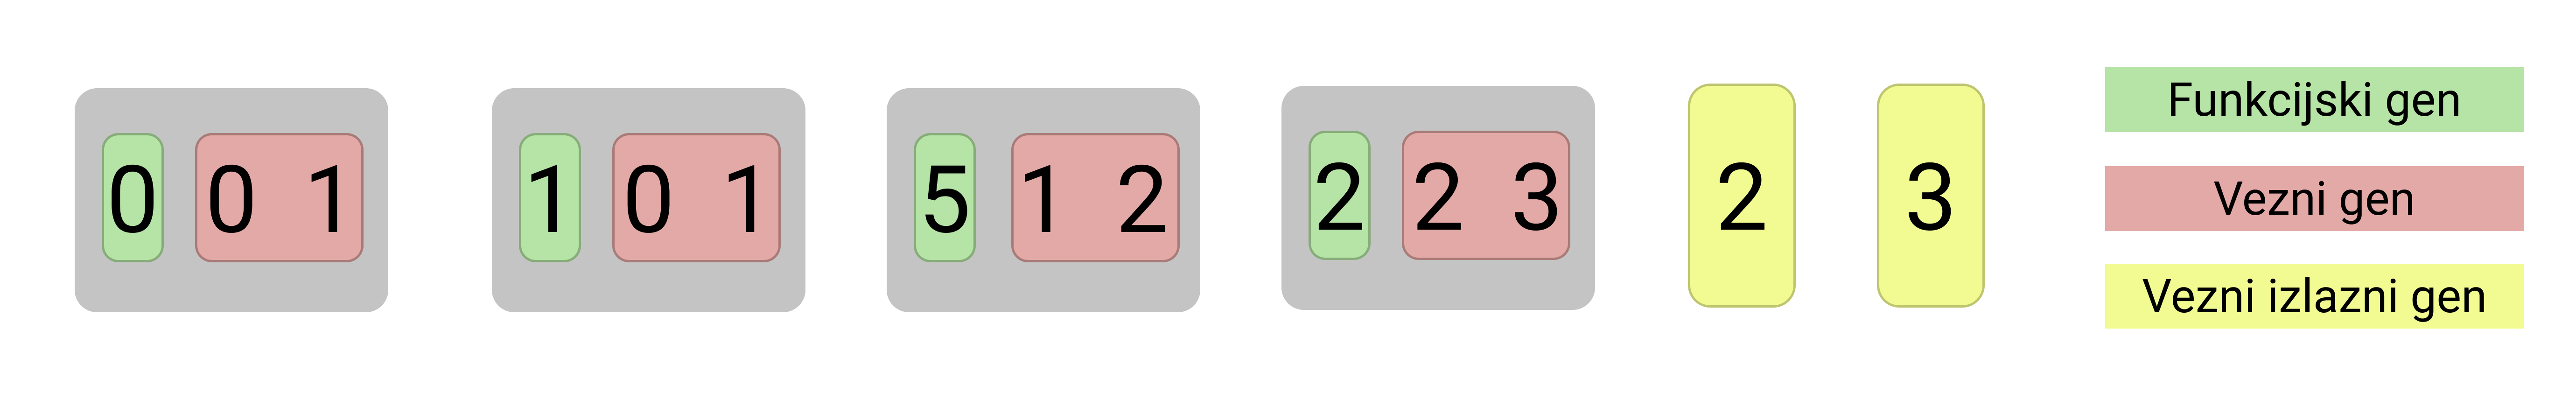
\includegraphics[width=\linewidth]{Illustrations/genotype.png}
	\caption{Primjer genotipa za CGP s dva ulaza, četiri sakrivena čvora i dva izlaza}
	\label{fig:genotype}
\end{figure}

\subsection{Arhitektura}
% Aciklički graf, dvodimenzionalnost, veličina, levelsback, nektivni čvor i kako utječe na fenotip
CGP jedinke prikazane su u obliku usmjerenih acikličnih grafova u dvodimenzionalnom prostoru (\cite{cgp}).
Arhitektura CGP jedinke definirana je sljedećim vrijednostima:
\begin{itemize}
	\item Broj ulaza $n_i$
	\item Broj izlaza $n_o$
	\item Broj skrivenih redaka i stupaca $n_r$ i $n_c$
	\item Broj najvećih vrijednost unazad koje čvor može uzimati (\emph{eng. levelsback}) $l$
\end{itemize}
Broj izlaza $>1$ nije tipična stvar za genetsko programiranje i veliki je benefit korištenja arhitekture inspirirane neuronskom mrežom.
Brojem najvećih vrijednosti unazad koje može čvor primiti definiramo složenost modela.
Priroda grafa takva je da se vrijednosti od prvog stupca šalju dublje sve do izlaza.
Ako je $l = 1$ definirali smo da svaki čvor može biti spojen najpliće u sloj prije sebe.
Tu mu dajemo manje slobode te ga ograničavamo na složenije modele, nego da smo dozvolili $l > 1$.
Naravno, ako želimo dozvoliti spajanje s čvorom iz bilo kojeg stupca, postavljamo  $l=n_c$.

Parametrima $n_r$ i $n_c$ definiramo broj računalnih čvorova kao $L_n = n_r \times n_c$.
Imajući to na umu, ne moraju svi čvorovi biti iskorišteni.
Čvorove koji ne vode prema izlazu nazivamo neaktivnim (\emph{eng. non-coding}).
Njihovi ulazi i funkcija nemaju nikakav utjecaj na konačni izlaz iz mreže.
Tu je vidljiva razlika između genotipa koji ima fiksnu i konstantnu duljinu i fenotipa čija duljina i oblik ovise o aktivnim i neaktivnim čvorovima.
Na slici \ref{fig:cgp_gene_feno} vidljiv je genotip CGP mreže i pripadajući fenotip s jasno označenim neaktivnim čvorovima i pravilima indeksiranja.

\begin{figure}
	\centering
	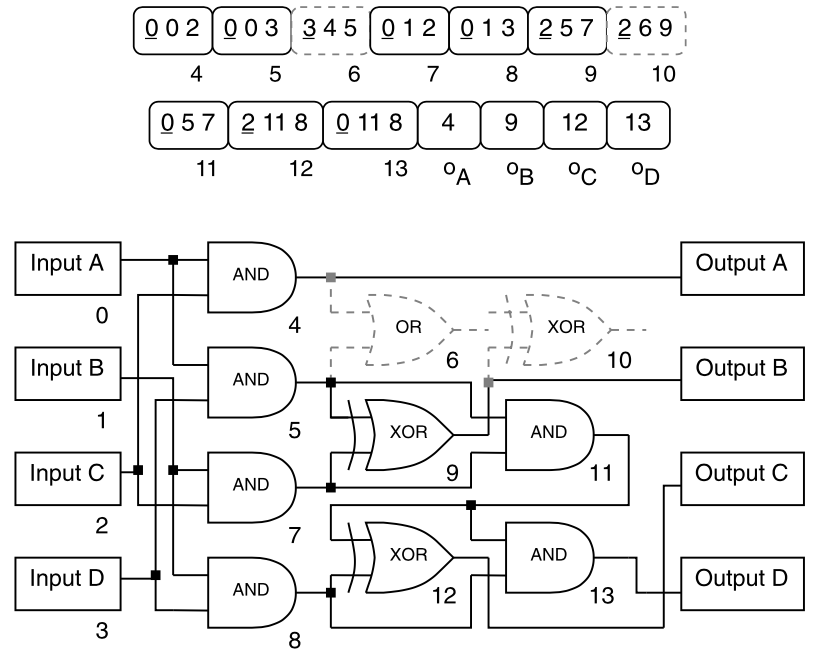
\includegraphics[width=\linewidth]{Illustrations/inactive_nodes.png}
	\caption{CGP genotip i fenotip digitalnog kruga. U čvorovima su vidljive funkcije koje izvode, a čvorovi koji su iscrtani su neaktivni jer ne vode ni na jedan izlaz. Također vidljivi su indeksi svakog čvora i u genotipu i fenotipu. Izvor \cite{cgp}}
	\label{fig:cgp_gene_feno}
\end{figure}

I u praksi i u tablici \ref{table:function_table} vidljivo je da nemaju sve funkcije jednak broj ulaza.
Na primjer, funkcija pod rednim brojem $4$, odnosno $\cos{x}$, ima jedan ulaz, dok funkcija $5$, $max(x, y)$ ima dva ulaza.
Treba li svakom čvoru dati točno onaj broj ulaza koliko traži njegova funkcija?
Naravno da ne, svako mutiranje mreže zahtjevalo bi ažuriranje broja ulaza u čvor i unijelo dodatnu kompleksnost u izvođenje te bi narušilo jednakost duljine genotipa svih jedinki.
Za svaku funkciju se zna njen broj ulaza (\emph{eng. arity}).
Ta vrijednost koristi se pri dodjeli broja ulaza čvorovima tako da svaki čvor dobije onoliko ulaza koliko prima funkcija s najvećim brojem ulaza.
Tako osiguravamo konstantnu duljinu genotipa i uklanjamo potrebu za ažuriranjem čvora pri promjeni funkcije iz npr. $cos{x}$ u $x + y$.

Prednost broja izlaza većeg od jedan vidljiva je na slici \ref{fig:cgp_gene_feno}.
Da se koristilo sintaksno stablo, bila bi potrebna četiri modela, jedan za svaki od izlaza A, B, C i D.
Velika prednost vidi se i u obradi slike.
\cite{conv_gp} predstavio je obradu slike konvolucijskim metodama, inače rezerviranim za neuronske mreže, genetskim programiranjem.
Koristeći predložene metode, za pokušaje izlučivanja $n$ značajki (\emph{eng. feature}), potrebno je koristiti $n$ sintaksnih stabala.
U slučaju korištenja CGP-a, dovoljna je samo jedna jedinka za sve značajke.

\subsection{Evoluiranje}

\subsubsection{Mutacija}
Mutacija u CGP genotipu mijenja vrijednost odabranog gena u drugu moguću vrijednost (\cite{cgp}).
Naglasak na moguću jer kao što je spomenuto, postoje funkcijski i vezni geni, svaki sa svojom domenom mogućih vrijednosti.
Mutacija se ne mora izvršiti jednom.
Stopa mutacije $\mu_r$ (\emph{eng. mutation rate}) zadana je od strane korisnika algoritma te uvjetuje pretragu prostora.
Najčešće se izražava kao postotak gena koji se mogu mutirati.
\cite{cgp} predlaže korištenje $1\%$ ili $0.01$ za jedinke s brojem čvorova $\leq 100$ za konzistentno dobre rezultate, što mogu i sam potvrditi u eksperimentima koji će biti navedeni u nastavku rada.
Ilustracija \ref{fig:cgp_mutation} prikazuje utjecaj mutiranja jednog veznog gena u genotipu.
\cite{cgp_experiment} pokazuje da u genotipima s $\approx 4000$ čvorova, postotak neaktivnih čvorova iznosi čak $95\%$.
Taj podatak, spojen s predloženom stopom mutacije unosi problem redundantne mutacije.
Reduntantna mutacija jest primjena mutacije na neaktivni čvor jer bez obzira promjenili vezu ili funkciju ne utječe na izlaz a samim time ni na kvalitetu CGP-a.
Iako \cite{cgp} adresira problem kao benefit jer nakon uspješnog mutiranja nakon više redundantnih nastaje višestruko mutirana jedinka, rezultati koje sam ja dobivao ne podupiru tu tvrdnju.
Pokušavajući povećati efikasnost algoritma, u vlastitoj implementaciji uzimao sam u obzir aktivnost, odnosno neaktivnost čvora te iste nisam uzimao u obzir.

\begin{figure}
	\centering
	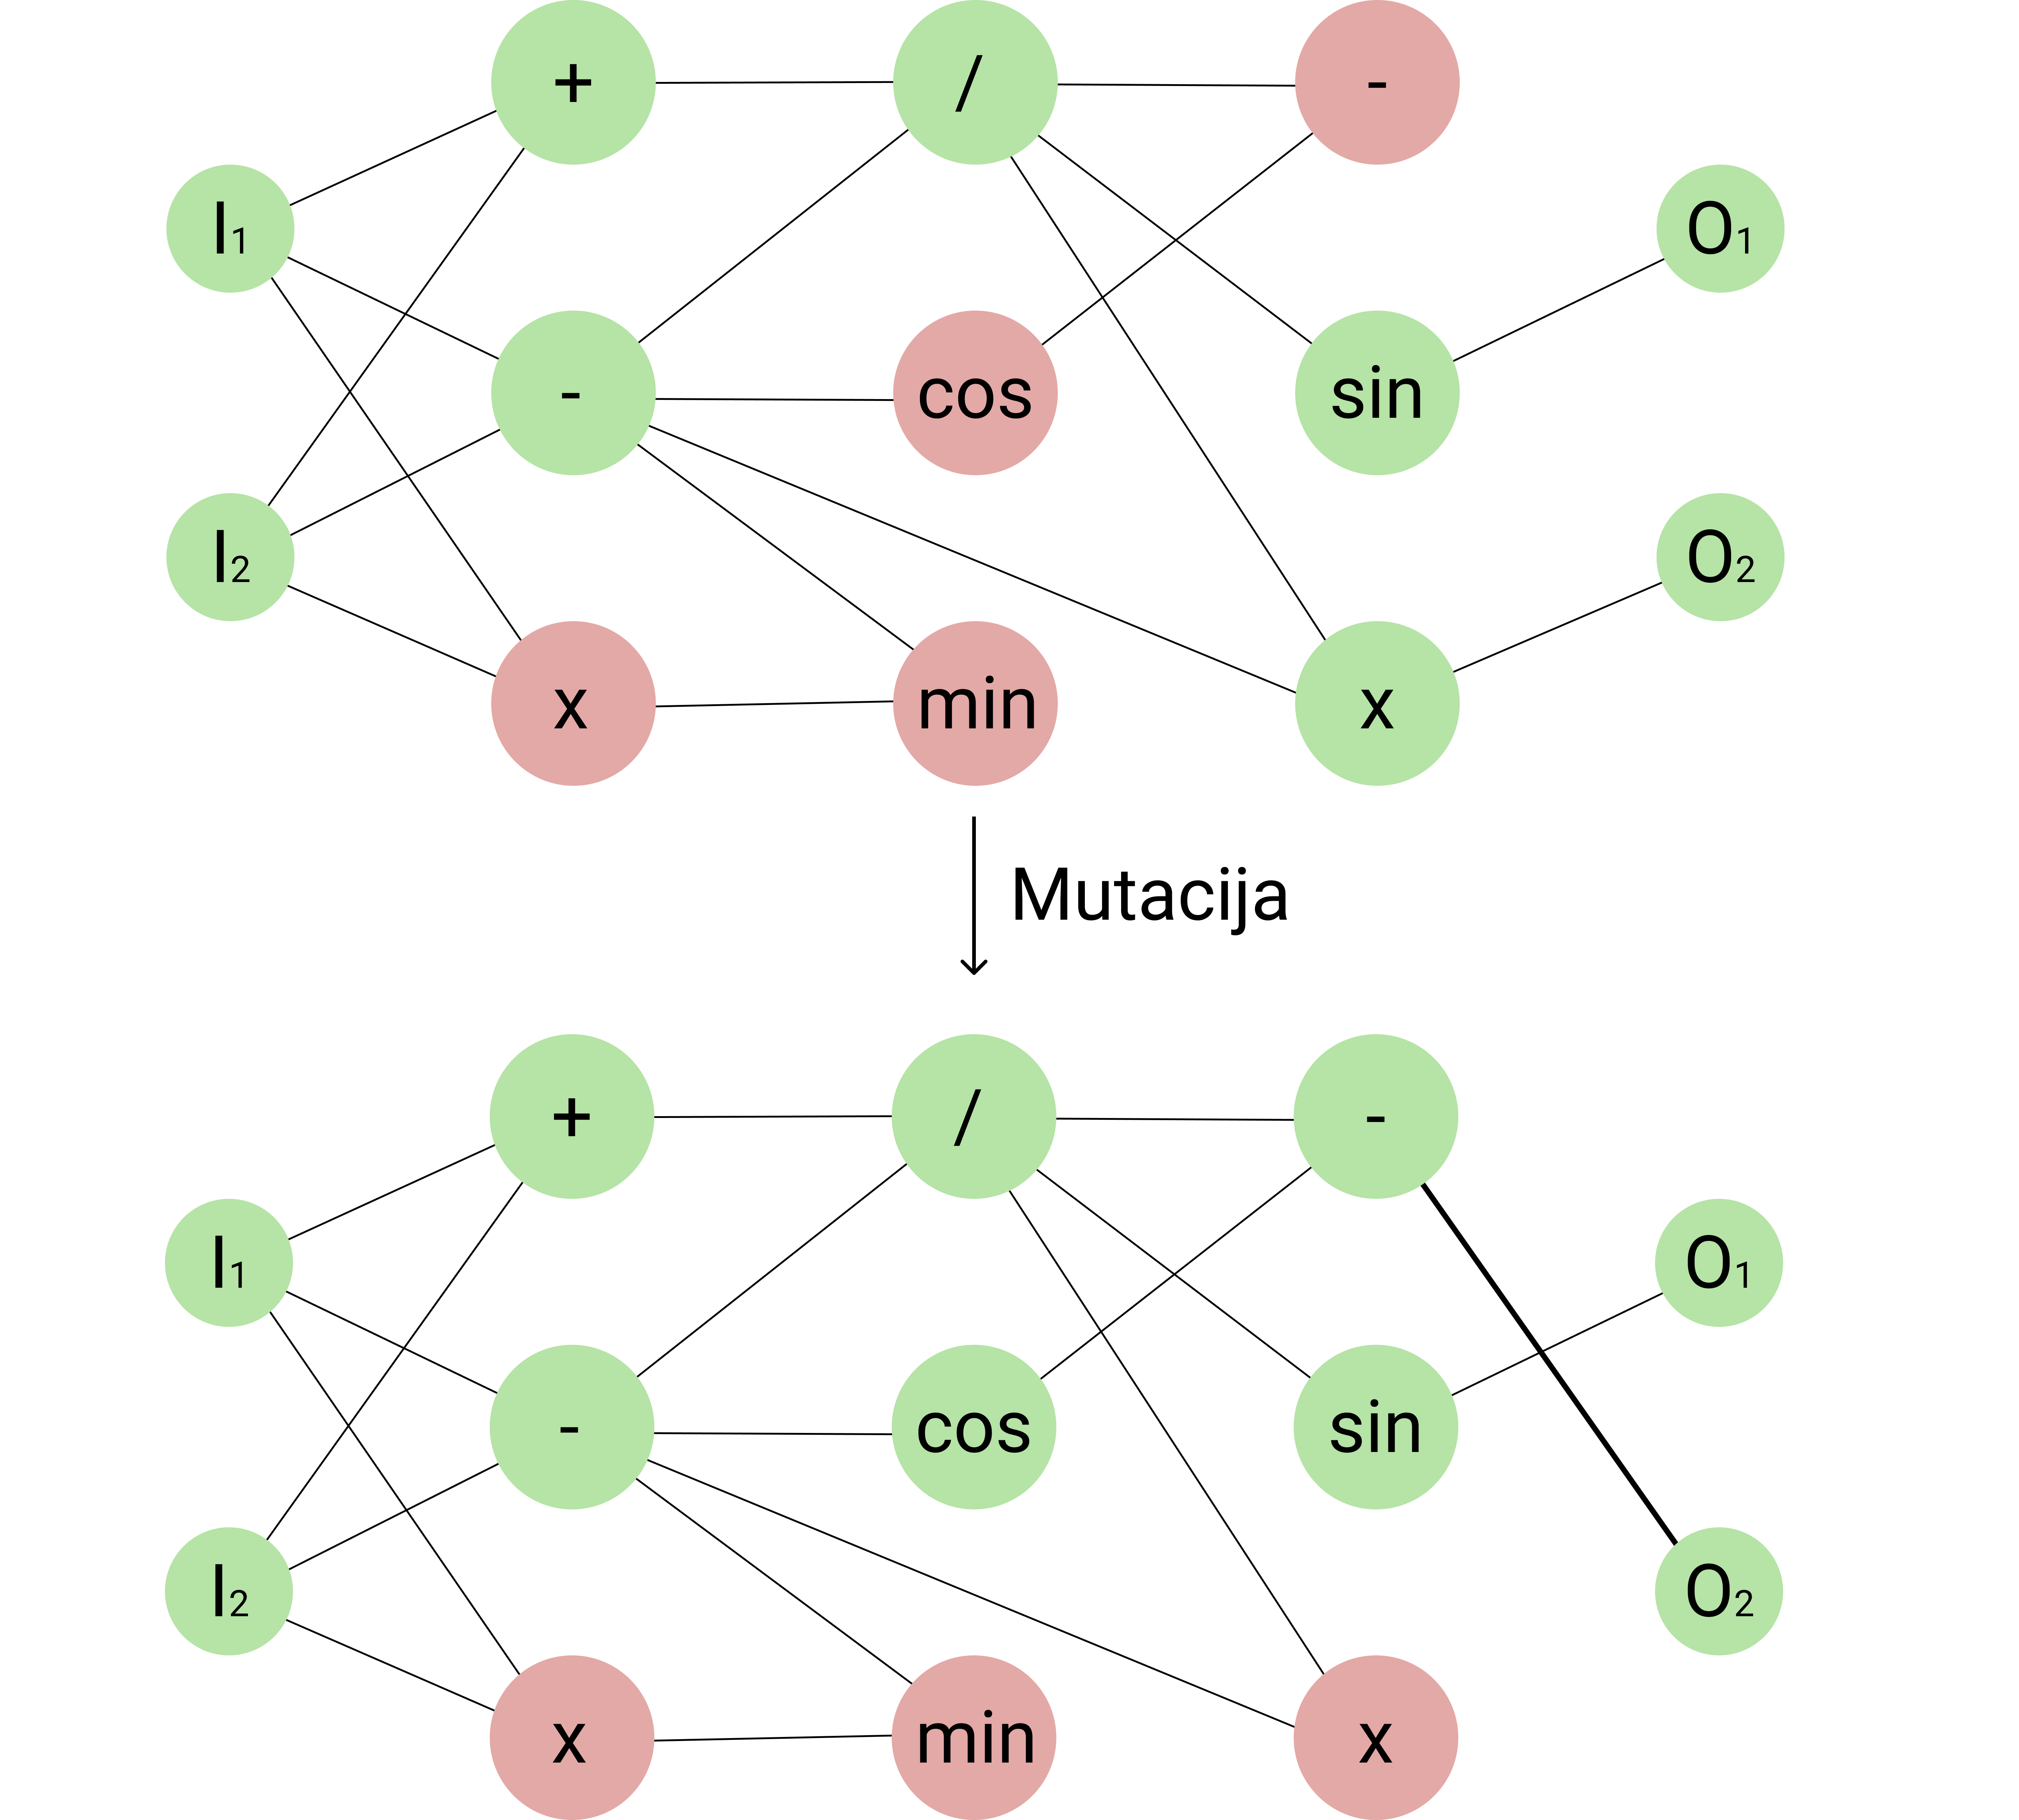
\includegraphics[width=\linewidth]{Illustrations/cgp_mutation.png}
	\caption{CGP fenotip prije i nakon mutacije. Aktivni, odnosno, neaktivni čvorovi jasno su naznačeni kao i novo-nastala veza.}
	\label{fig:cgp_mutation}
\end{figure}

\subsubsection{Križanje}
Kao što je spomenuto, genotip je vektor cijelih brojeva fiksne duljine.
Velika prednost toga je što je križanje iznimno lako za ostvariti.
Za razliku od mutacije, ne moramo paziti na domene pojedinih gena.
Operator križanja koji se koristi je križanje u $k$ točaka gdje je $k = 1$.
Iako je lako izvodivo, sa sobom nosi nedostatke.
Rezultat križanja je spajanje dva podgrafa koja zajedno daju lošije rezultate nego dva originalna CGP-a zasebno.
\cite{cgp_experiment} predstavlja nekolicinu radova s obečavajućim rezultatima koristeći eksperimentalne načine križanja, no istraživanje i isprobavanje istih nije u sklopu ovog rada.

\subsubsection{Algoritam}
Algoritam evolucije koji predlaže \cite{cgp} je $1 + \lambda$.
$\lambda$ može biti proizvoljna vrijednost koja predstavlja broj potomaka nastalih mutacijom.
Spomenuti rad predlaže korištenje $\lambda = 4$.
Rezultati eksperimenata koji će biti prikazani u nastavku potvrđuju tu tvrdnju iako sam mjestimično koristio $\lambda = 8$ kao što predlaže \cite{Sekanina2011}.
Evolucija je detaljnije prikazana algoritmom \ref{alg:cgp_evolution}.

\begin{algorithm}
	\caption{Strategija $1 + \lambda$ za evoluciju CGP-a}
	\label{alg:cgp_evolution}
	\begin{algorithmic}
		\FOR{i unutar $0 \leq i \leq \lambda$}
			\STATE Stvori $CGP_i$
		\ENDFOR
		\STATE Od stvorenih CGP odaberi najbolji i definiraj ga kao roditelja
		\WHILE{uvjet zaustavljanja nije ostvaren}
			\FOR{i unutar $0 \leq i < \lambda$}
				\STATE Mutiraj roditelja i stvori novi $CGP_i$
			\ENDFOR
			\STATE Evaluiraj nove potomke i odaberi najbolji
			\IF{najbolji potomak pokazuje bolje ili jednako ponašanje nego roditelj}
				\STATE Roditelj $\leftarrow$ Najbolji potomak
			\ENDIF
		\ENDWHILE
	\end{algorithmic}
\end{algorithm}
